\section{Experiments}\label{s:experiments}
% \begin{table*}[h]
% \TopFloatBoxes
% \thisfloatsetup{subfloatrowsep=none}
% \setlength{\tabcolsep}{2.5pt}
% \begin{floatrow}
% \floatbox[\nocapbeside]{table}[\FBwidth]
% {
% \caption{\textbf{Unsupervised image clustering (IID).} $\dagger$: method based on k-means. $\ddagger$: method that does not directly learn a clustering function and requires further application of k-means to be used for image clustering. $\star$: results obtained using our experiments with authors' original code.}\label{t:img_clus_iid}
% }
% {
% \setlength{\tabcolsep}{2.5pt}
% \fontsize{8}{9}\selectfont 
% \begin{tabular}{lcccc}
% \toprule
% & STL10 & CIFAR10 & CIFAR100-20 & MNIST \\
% \midrule
% Random network & 13.5 & 13.1 & 5.93 & 26.1 \\
% K-means~\cite{zelnik2005self}$\dagger$  & 19.2 & 22.9 & 13.0 & 57.2 \\
% Spectral clustering~\cite{wang2015optimized} & 15.9 & 24.7 & 13.6 & 69.6\\
% AE~\cite{bengio2007greedy}$\ddagger$ & 30.3 & 31.4 & 16.5 & 81.2 \\
% Sparse AE~\cite{ng2011sparse}$\ddagger$ & 32.0 & 29.7 & 15.7 & 82.7\\
% Denoising AE~\cite{vincent2010stacked}$\ddagger$ & 30.2 & 29.7 & 15.1 & 83.2\\
% Variational Bayes AE~\cite{kingma2013auto}$\ddagger$ & 28.2 & 29.1 & 15.2 & 83.2\\
% SWWAE 2015~\cite{zhao1506stacked}$\ddagger$ & 27.0 & 28.4 & 14.7 & 82.5 \\
% GAN 2015~\cite{radford2015unsupervised}$\ddagger$ & 29.8 & 31.5 & 15.1 & 82.8\\
% JULE 2016~\cite{yang2016joint}$\ddagger$ & 27.7 & 27.2 & 13.7 & 96.4 \\
% DEC 2016~\cite{xie2016unsupervised}$\dagger$ $\ddagger$ & 35.9 & 30.1 & 18.5 & 84.3 \\
% DAC 2017~\cite{chang2017deep} & 47.0 & 52.2 & 23.8 & 97.8 \\
% %(IMSAT 2017) & - & - & - & 98.4 \\
% DeepCluster 2018~\cite{caron2018deep}$\dagger$ $\ddagger$ & 33.4$\star$ & 37.4$\star$ & 18.9$\star$ & 65.6 $\star$ \\
% ADC 2018~\cite{haeusser18associative} & 53.0 & 32.5 & 16.0$\star$ & 99.2 \\
% IID (best sub-head) & \textbf{60.4} \cmt{247} & \textbf{61.3} \cmt{256} &\textbf{24.4} \cmt{269} & \textbf{99.3} \cmt{258} \\
% IID (avg sub-head $\pm$ std) & \textbf{56.7 $\pm$ 3.03} \cmt{247} & \textbf{61.3 $\pm$ 0.010} \cmt{256} &\textbf{24.0 $\pm$ 0.311} \cmt{269} & \textbf{99.3 $\pm$ 0.003} \cmt{258} \\
% \midrule
% IID+ (overclustering) & 61.4 & 62.9 & 33.6 & 98.9 \\
% \bottomrule
% \end{tabular}}%
% \floatbox[\nocapbeside]{table}[\FBwidth]
% {
% \caption{\textbf{Ablation} for IID. Each row contains one change from the full setting with all else equal. Full setting: with auxiliary overclustering, 5 initialisation heads, 5 sample repeats, unlabelled data segment used.}
% }
% {
% \footnotesize    
% \begin{tabular}{lc}
% \toprule
% & STL10 \\
% \midrule
% No auxiliary overclustering & 39.9 \cmt{418}\\
% Single sub-head ($h=1$) & 50.7\cmt{419}\\
% No sample repeats ($r=1$) & 51.4\cmt{420}\\
% Unlabelled data segment ignored & 50.5\cmt{421}\\
% \midrule
% Full setting & \textbf{60.4} \cmt{247}\\
% \bottomrule
% \end{tabular}
% }
% \end{floatrow}
% \end{table*}


% \begin{table*}
% \TopFloatBoxes
% \thisfloatsetup{subfloatrowsep=none}
% \begin{floatrow}
% \floatbox[\nocapbeside]{table}[\FBwidth]
% {
% \caption{\textbf{Unsupervised image clustering (IID).} $\dagger$: method based on k-means. $\ddagger$: method that does not directly learn a clustering function and requires further application of k-means to be used for image clustering. $\star$: results obtained using our experiments with authors' original code.}\label{t:img_clus_iid}
% }
% {
% \setlength{\tabcolsep}{2.5pt}
% \fontsize{8}{9}\selectfont 
% \begin{tabular}{lcccc}
% \toprule
% & STL10 & CIFAR10 & CFR100-20 & MNIST \\
% \midrule
% Random network & 13.5 & 13.1 & 5.93 & 26.1 \\
% K-means~\cite{zelnik2005self}$\dagger$  & 19.2 & 22.9 & 13.0 & 57.2 \\
% Spectral clustering~\cite{wang2015optimized} & 15.9 & 24.7 & 13.6 & 69.6\\
% AE~\cite{bengio2007greedy}$\ddagger$ & 30.3 & 31.4 & 16.5 & 81.2 \\
% Sparse AE~\cite{ng2011sparse}$\ddagger$ & 32.0 & 29.7 & 15.7 & 82.7\\
% Denoising AE~\cite{vincent2010stacked}$\ddagger$ & 30.2 & 29.7 & 15.1 & 83.2\\
% Variational Bayes AE~\cite{kingma2013auto}$\ddagger$ & 28.2 & 29.1 & 15.2 & 83.2\\
% SWWAE 2015~\cite{zhao1506stacked}$\ddagger$ & 27.0 & 28.4 & 14.7 & 82.5 \\
% GAN 2015~\cite{radford2015unsupervised}$\ddagger$ & 29.8 & 31.5 & 15.1 & 82.8\\
% JULE 2016~\cite{yang2016joint}$\ddagger$ & 27.7 & 27.2 & 13.7 & 96.4 \\
% DEC 2016~\cite{xie2016unsupervised}$\dagger$ $\ddagger$ & 35.9 & 30.1 & 18.5 & 84.3 \\
% DAC 2017~\cite{chang2017deep} & 47.0 & 52.2 & 23.8 & 97.8 \\
% %(IMSAT 2017) & - & - & - & 98.4 \\
% DeepCluster 2018~\cite{caron2018deep}$\dagger$ $\ddagger$ & 33.4$\star$ & 37.4$\star$ & 18.9$\star$ & 65.6 $\star$ \\
% ADC 2018~\cite{haeusser18associative} & 53.0 & 32.5 & 16.0$\star$ & 99.2 \\
% IID (best sub-head) & \textbf{60.4} \cmt{247} & \textbf{61.3} \cmt{256} &\textbf{24.4} \cmt{269} & \textbf{99.3} \cmt{258} \\
% IID (avg sub-head $\pm$ std. dev.) & \textbf{56.7} \cmt{247} & \textbf{61.3} \cmt{256} &\textbf{24.0} \cmt{269} & \textbf{99.3} \cmt{258} \\[-0.2em]
%  & ~~\scriptsize\textbf{$\pm$ 3.03} \cmt{247} & \scriptsize\textbf{$\pm$ 0.010} \cmt{256} & \scriptsize\textbf{$\pm$ 0.311} \cmt{269} & \scriptsize\textbf{$\pm$ 0.003} \cmt{258} \\
% \midrule
% IID+ (overclustering) & 61.4 & 62.9 & 33.6 & 98.9 \\
% \bottomrule
% \end{tabular}}%
% \floatbox[\nocapbeside]{table}[\FBwidth]
% {
% \caption{\textbf{Ablation} for IID. Each row contains one change from the full setting with all else equal. Full setting: with auxiliary overclustering, 5 initialisation heads, 5 sample repeats, unlabelled data segment used.}
% }
% {
% \footnotesize    
% \begin{tabular}{lc}
% \toprule
% & STL10 \\
% \midrule
% No auxiliary overclustering & 39.9 \cmt{418}\\
% Single sub-head ($h=1$) & 50.7\cmt{419}\\
% No sample repeats ($r=1$) & 51.4\cmt{420}\\
% Unlabelled data segment ignored & 50.5\cmt{421}\\
% \midrule
% Full setting & \textbf{60.4} \cmt{247}\\
% \bottomrule
% \end{tabular}
% }
% \end{floatrow}
% \end{table*}

\begin{table}[t]
\setlength{\tabcolsep}{2.5pt}
\fontsize{8}{9}\selectfont 
\begin{tabular}{lcccc}
\toprule
& STL10 & CIFAR10 & CFR100-20 & MNIST \\
\midrule
Random network & 13.5 & 13.1 & 5.93 & 26.1 \\
K-means~\cite{zelnik2005self}$\dagger$  & 19.2 & 22.9 & 13.0 & 57.2 \\
Spectral clustering~\cite{wang2015optimized} & 15.9 & 24.7 & 13.6 & 69.6\\
Triplets~\cite{schultz2004learning}$\ddagger$ & 24.4 & 20.5 & 9.94 & 52.5 \\
AE~\cite{bengio2007greedy}$\ddagger$ & 30.3 & 31.4 & 16.5 & 81.2 \\
Sparse AE~\cite{ng2011sparse}$\ddagger$ & 32.0 & 29.7 & 15.7 & 82.7\\
Denoising AE~\cite{vincent2010stacked}$\ddagger$ & 30.2 & 29.7 & 15.1 & 83.2\\
Variational Bayes AE~\cite{kingma2013auto}$\ddagger$ & 28.2 & 29.1 & 15.2 & 83.2\\
SWWAE 2015~\cite{zhao2015stacked}$\ddagger$ & 27.0 & 28.4 & 14.7 & 82.5 \\
GAN 2015~\cite{radford2015unsupervised}$\ddagger$ & 29.8 & 31.5 & 15.1 & 82.8\\
JULE 2016~\cite{yang2016joint} & 27.7 & 27.2 & 13.7 & 96.4 \\
DEC 2016~\cite{xie2016unsupervised}$\dagger$ & 35.9 & 30.1 & 18.5 & 84.3 \\
DAC 2017~\cite{chang2017deep} & 47.0 & 52.2 & 23.8 & 97.8 \\
%(IMSAT 2017) & - & - & - & 98.4 \\
DeepCluster 2018~\cite{caron2018deep}$\dagger$ $\ddagger$ & 33.4$\star$ & 37.4$\star$ & 18.9$\star$ & 65.6 $\star$ \\
ADC 2018~\cite{haeusser2018associative} & 53.0 & 32.5 & 16.0$\star$ & 99.2 \\
\midrule
  \methodnameshort (lowest loss sub-head) & \textbf{59.6} \cmt{569} & \textbf{61.7} \cmt{640} &\textbf{25.7} \cmt{579} & \textbf{99.2} \cmt{685} \\
\methodnameshort (avg sub-head $\pm$ STD) & 59.8 & 57.6 & 25.5 & 98.4 \\[-0.2em]
  & ~~\scriptsize$\pm$ 0.844 & \scriptsize$\pm$ 5.01 & \scriptsize$\pm$ 0.462 & \scriptsize$\pm$ 0.652 \\
\bottomrule
\end{tabular}
\caption{\textbf{Unsupervised image clustering.} Legend: $\dagger$Method based on k-means. $\ddagger$Method that does not directly learn a clustering function and requires further application of k-means to be used for image clustering. $\star$Results obtained using our experiments with authors' original code.}\label{t:img_clus_iid}
\end{table}


\begin{comment}
  \methodnameshort (best sub-head) & \textbf{61.0} \cmt{569} & \textbf{61.7} \cmt{640} &\textbf{25.7} \cmt{579} & \textbf{99.3} \cmt{685} \\
\methodnameshort (avg sub-head $\pm$ STD) & 59.8 & 57.6 & 25.5 & 98.4 \\[-0.2em]
  & ~~\scriptsize$\pm$ 0.844 & \scriptsize$\pm$ 5.01 & \scriptsize$\pm$ 0.462 & \scriptsize$\pm$ 0.652 \\
\end{comment}
  
\begin{table}[t]
\footnotesize    
\begin{tabular}{lc}
\toprule
& STL10 \\
\midrule
No auxiliary overclustering & 43.8 \cmt{692}\\
Single sub-head ($h=1$) & 57.6\cmt{693}\\
No sample repeats ($r=1$) & 47.0\cmt{694}\\
Unlabelled data segment ignored & 49.9\cmt{695}\\
\midrule
Full setting & \textbf{59.6} \cmt{569}\\
\bottomrule
\end{tabular}
\caption{\textbf{Ablations of \methodnameshort (unsupervised setting).} Each row shows a single change from the full setting. The full setting has auxiliary overclustering, 5 initialisation heads, 5 sample repeats, and uses the unlabelled data subset of STL10.}
\label{t:iid_imgclus_ablation}
\end{table}

% \begin{table}[h]
% \footnotesize 
% \begin{center}
% \begin{tabular}{lc}
% \toprule
% & STL10 \\
% \midrule
% No auxiliary overclustering & 39.9 \cmt{418}\\
% Single sub-head ($h=1$) & 50.7\cmt{419}\\
% No sample repeats ($r=1$) & 51.4\cmt{420}\\
% Unlabelled data segment ignored & 50.5\cmt{421}\\
% \midrule
% Full setting & \textbf{60.4} \cmt{247}\\
% \bottomrule
% \end{tabular}
% \end{center}
% \vspace{-1em}
% \caption{Ablation for IID. Each row contains one change from the full setting with all else equal. Full setting: with auxiliary overclustering, 5 initialisation heads, 5 sample repeats, unlabelled data segment used.}
% \label{t:iid_imgclus_ablation}
% \end{table}

We apply \methodnameshort to fully unsupervised image clustering and segmentation, as well as two semi-supervised settings. Existing baselines are outperformed in all cases.
We also conduct an analysis of our method via ablation studies. For minor details see supplementary material.

\subsection{Image clustering}\label{s:exp_img_clus}
\begin{figure*}[t]
\begin{center}
\setlength\tabcolsep{1.5pt} % default value: 6pt
\begin{tabular}{c c c c c c c c c c c c c c c c}
\multicolumn{2}{c}{\textbf{\textit{Cat}}} &  
\multicolumn{2}{c}{\textbf{\textit{Dog}}} &
\multicolumn{2}{c}{\textbf{\textit{Bird}}} &
\multicolumn{2}{c}{\textbf{\textit{Deer}}} &
\multicolumn{2}{c}{\textbf{\textit{Monkey}}} &
\multicolumn{2}{c}{\textbf{\textit{Car}}} &
\multicolumn{2}{c}{\textbf{\textit{Plane}}} &
\multicolumn{2}{c}{\textbf{\textit{Truck}}} \\

%1st

\includegraphics[width=0.055\textwidth]{experiments2_files/3222_img.png} &
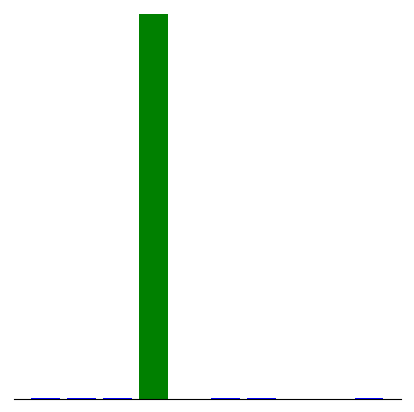
\includegraphics[width=0.055\textwidth]{experiments2_files/3222_pred.png} &

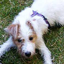
\includegraphics[width=0.055\textwidth]{experiments2_files/1667_img.png} &
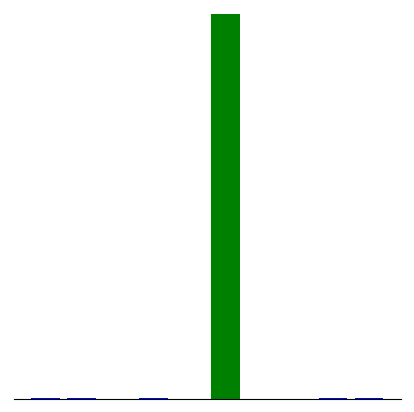
\includegraphics[width=0.055\textwidth]{experiments2_files/1667_pred.png} &

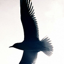
\includegraphics[width=0.055\textwidth]{experiments2_files/2701_img.png} &
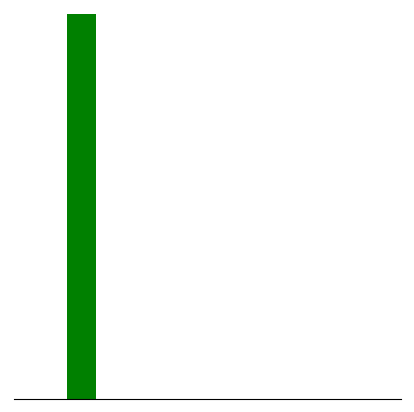
\includegraphics[width=0.055\textwidth]{experiments2_files/2701_pred.png} &

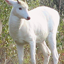
\includegraphics[width=0.055\textwidth]{experiments2_files/1996_img.png} &
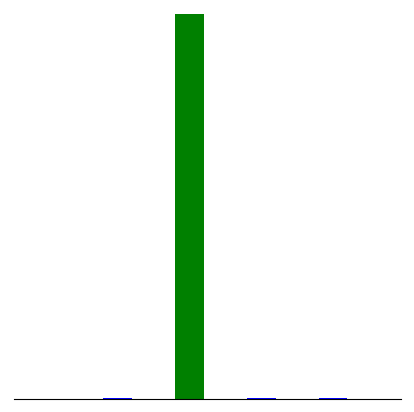
\includegraphics[width=0.055\textwidth]{experiments2_files/1996_pred.png} &

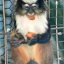
\includegraphics[width=0.055\textwidth]{experiments2_files/4284_img.png} &
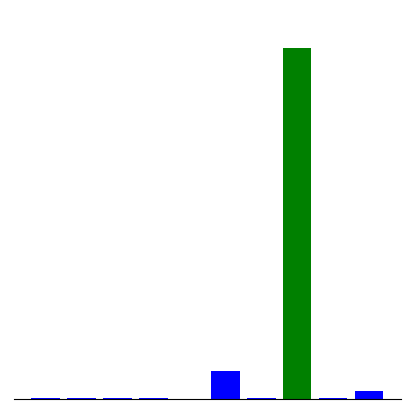
\includegraphics[width=0.055\textwidth]{experiments2_files/4284_pred.png} &


\includegraphics[width=0.055\textwidth]{experiments2_files/6750_img.png} &
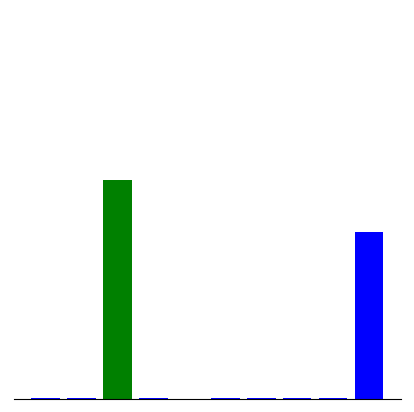
\includegraphics[width=0.055\textwidth]{experiments2_files/6750_pred.png} &


\includegraphics[width=0.055\textwidth]{experiments2_files/10930_img.png} &
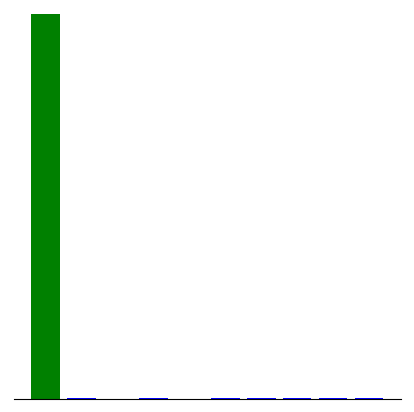
\includegraphics[width=0.055\textwidth]{experiments2_files/10930_pred.png} &

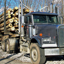
\includegraphics[width=0.055\textwidth]{experiments2_files/2612_img.png} &
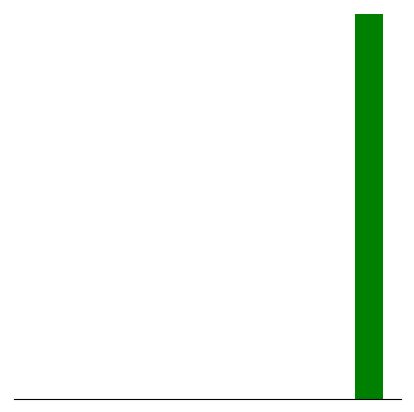
\includegraphics[width=0.055\textwidth]{experiments2_files/2612_pred.png} \\

% 2nd
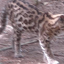
\includegraphics[width=0.055\textwidth]{experiments2_files/7006_img.png} &
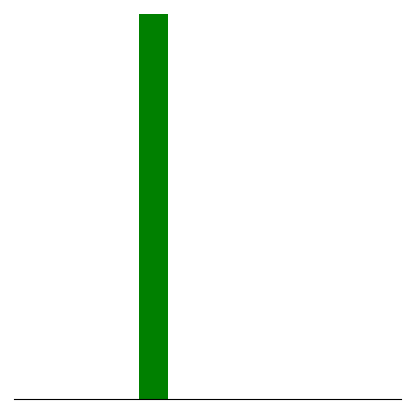
\includegraphics[width=0.055\textwidth]{experiments2_files/7006_pred.png} &

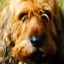
\includegraphics[width=0.055\textwidth]{experiments2_files/1255_img.png} &
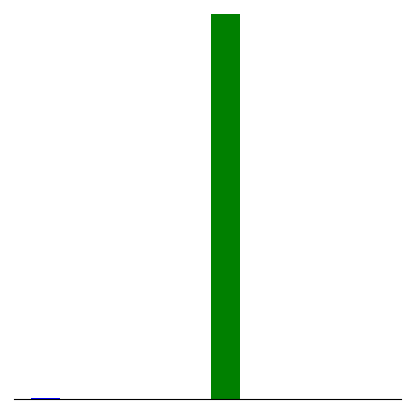
\includegraphics[width=0.055\textwidth]{experiments2_files/1255_pred.png} &

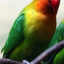
\includegraphics[width=0.055\textwidth]{experiments2_files/2428_img.png} &
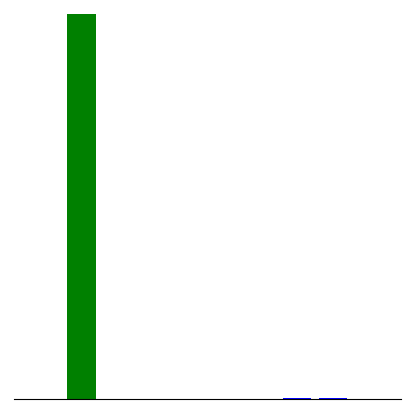
\includegraphics[width=0.055\textwidth]{experiments2_files/2428_pred.png} &

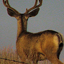
\includegraphics[width=0.055\textwidth]{experiments2_files/3374_img.png} &
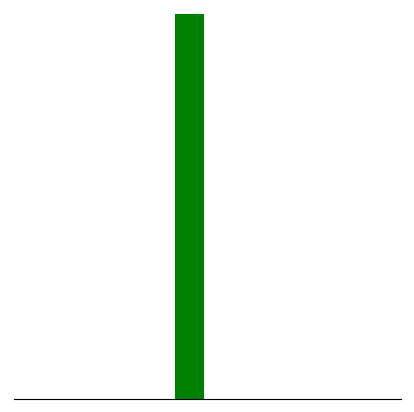
\includegraphics[width=0.055\textwidth]{experiments2_files/3374_pred.png} &

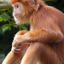
\includegraphics[width=0.055\textwidth]{experiments2_files/7112_img.png} &
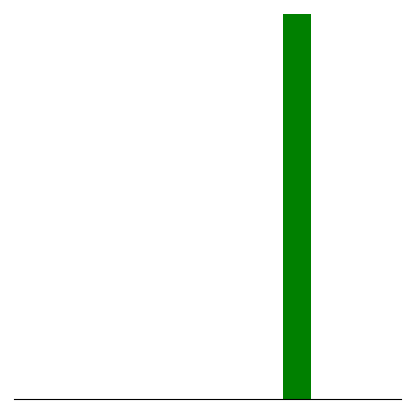
\includegraphics[width=0.055\textwidth]{experiments2_files/7112_pred.png} &

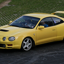
\includegraphics[width=0.055\textwidth]{experiments2_files/12904_img.png} &
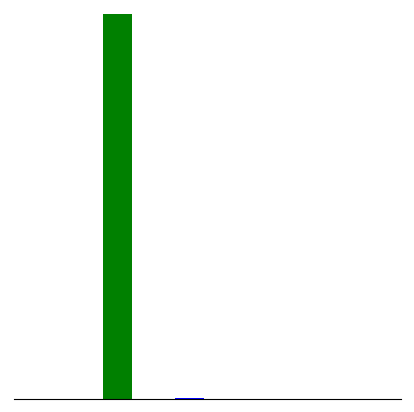
\includegraphics[width=0.055\textwidth]{experiments2_files/12904_pred.png} &

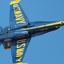
\includegraphics[width=0.055\textwidth]{experiments2_files/9944_img.png} &
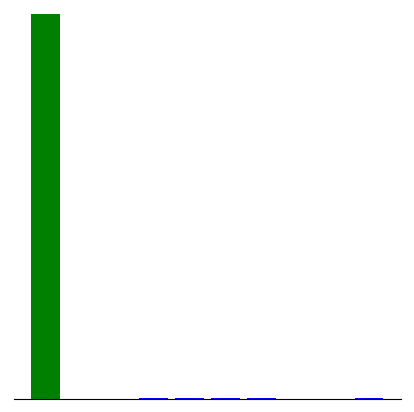
\includegraphics[width=0.055\textwidth]{experiments2_files/9944_pred.png} &

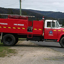
\includegraphics[width=0.055\textwidth]{experiments2_files/6340_img.png} &
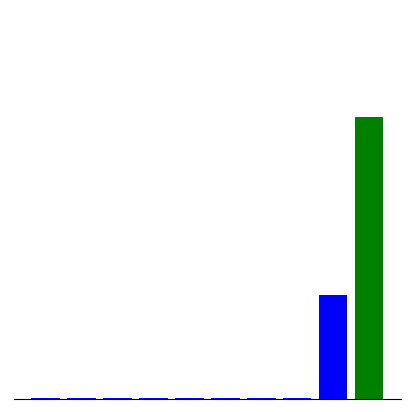
\includegraphics[width=0.055\textwidth]{experiments2_files/6340_pred.png} \\

% 3rd

\includegraphics[width=0.055\textwidth]{experiments2_files/7790_img.png} &
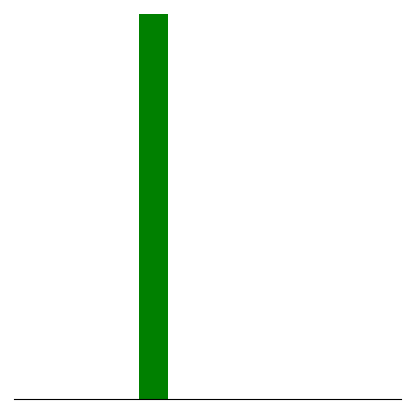
\includegraphics[width=0.055\textwidth]{experiments2_files/7790_pred.png} &

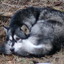
\includegraphics[width=0.055\textwidth]{experiments2_files/8345_img.png} &
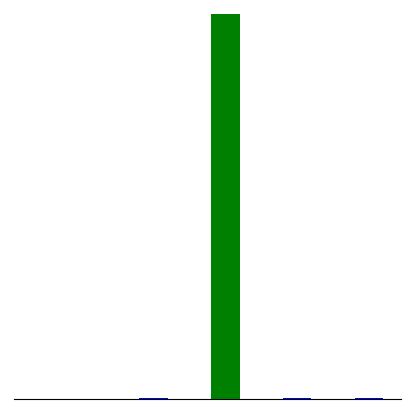
\includegraphics[width=0.055\textwidth]{experiments2_files/8345_pred.png} &

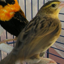
\includegraphics[width=0.055\textwidth]{experiments2_files/12056_img.png} &
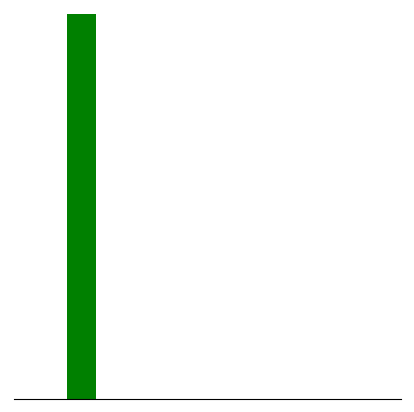
\includegraphics[width=0.055\textwidth]{experiments2_files/12056_pred.png} &

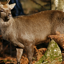
\includegraphics[width=0.055\textwidth]{experiments2_files/1752_img.png} &
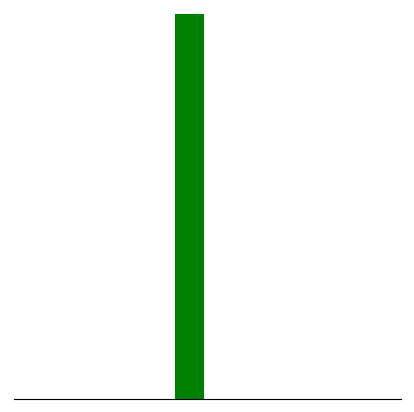
\includegraphics[width=0.055\textwidth]{experiments2_files/1752_pred.png} &

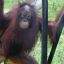
\includegraphics[width=0.055\textwidth]{experiments2_files/11217_img.png} &
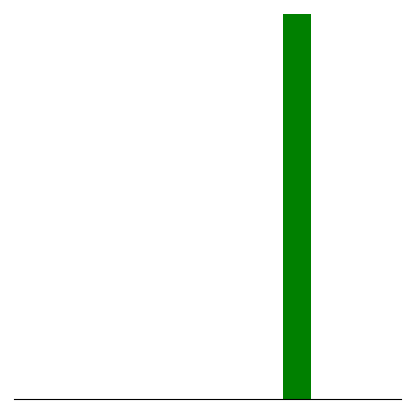
\includegraphics[width=0.055\textwidth]{experiments2_files/11217_pred.png} &


\includegraphics[width=0.055\textwidth]{experiments2_files/11856_img.png} &
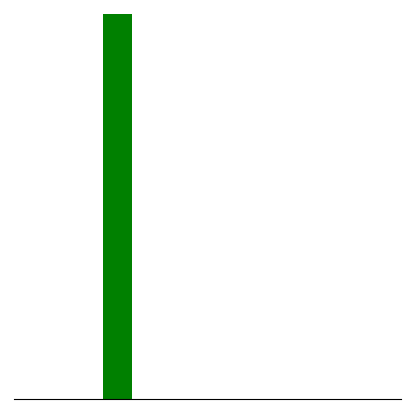
\includegraphics[width=0.055\textwidth]{experiments2_files/11856_pred.png} &


\includegraphics[width=0.055\textwidth]{experiments2_files/7190_img.png} &
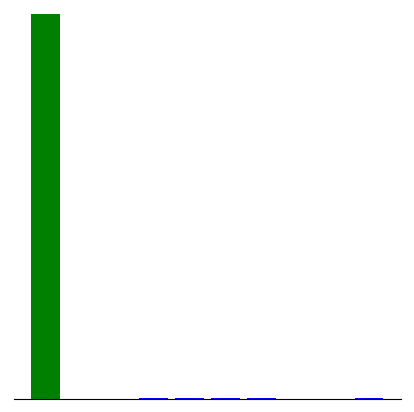
\includegraphics[width=0.055\textwidth]{experiments2_files/7190_pred.png} &


\includegraphics[width=0.055\textwidth]{experiments2_files/6350_img.png} &
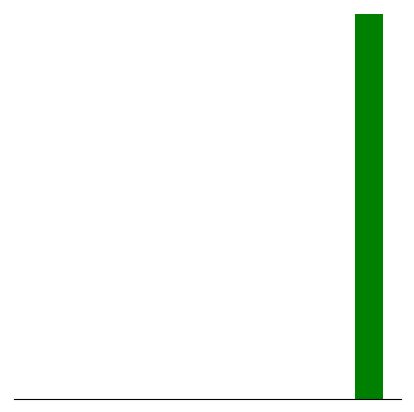
\includegraphics[width=0.055\textwidth]{experiments2_files/6350_pred.png} \\

% 4th
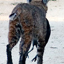
\includegraphics[width=0.055\textwidth]{experiments2_files/3703_img.png} &
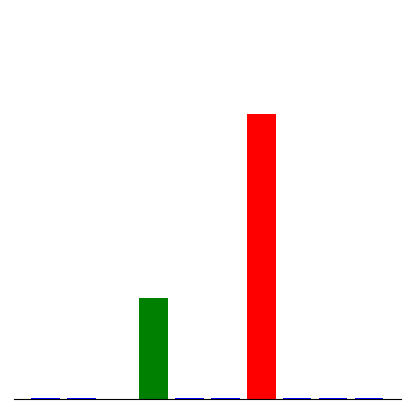
\includegraphics[width=0.055\textwidth]{experiments2_files/3703_pred.png} &

\includegraphics[width=0.055\textwidth]{experiments2_files/7823_img.png} &
\includegraphics[width=0.055\textwidth]{experiments2_files/7823_pred.png} &

\includegraphics[width=0.055\textwidth]{experiments2_files/7794_img.png} &
\includegraphics[width=0.055\textwidth]{experiments2_files/7794_pred.png} &

\includegraphics[width=0.055\textwidth]{experiments2_files/6957_img.png} &
\includegraphics[width=0.055\textwidth]{experiments2_files/6957_pred.png} &

\includegraphics[width=0.055\textwidth]{experiments2_files/5464_img.png} &
\includegraphics[width=0.055\textwidth]{experiments2_files/5464_pred.png} &

\includegraphics[width=0.055\textwidth]{experiments2_files/12265_img.png} &
\includegraphics[width=0.055\textwidth]{experiments2_files/12265_pred.png} &

\includegraphics[width=0.055\textwidth]{experiments2_files/12430_img.png} &
\includegraphics[width=0.055\textwidth]{experiments2_files/12430_pred.png} &

\includegraphics[width=0.055\textwidth]{experiments2_files/2778_img.png} &
\includegraphics[width=0.055\textwidth]{experiments2_files/2778_pred.png} \\
\end{tabular}
\end{center}\vspace{-1em}
\caption{\textbf{Unsupervised image clustering (\methodnameshort) results on STL10.} Predicted cluster probabilities from the best performing head are shown as bars. Prediction corresponds to tallest, ground truth is green, incorrectly predicted classes are red, and all others are blue. The bottom row shows failure cases.}
\label{f:images_img_clus}
\end{figure*}
\begin{figure*}[t]
\TopFloatBoxes
\begin{floatrow}
\floatbox[\nocapbeside]{table}[0.27\textwidth]  %\FBwidth
{
\caption{\textbf{Fully and semi-supervised classification.} Legend: *Fully supervised method. $\star$Our experiments with authors' code. $\dagger$Multi-fold evaluation.}%training where average over training folds is reported (others use the full training set).
\label{t:iid_imgclus_semisup}
}
{
\scriptsize
\begin{tabular}{lc}
\toprule
& STL10 \\
\midrule
Dosovitskiy 2015~\cite{dosovitskiy2015discriminative}$\dagger$ & 74.2 \\
SWWAE 2015~\cite{zhao2015stacked}$\dagger$ & 74.3 \\
Dundar 2015~\cite{dundar2015convolutional}& 74.1 \\
Cutout* 2017~\cite{devries2017improved}& 87.3 \\
Oyallon* 2017~\cite{oyallon2017scaling}$\dagger$ & 76.0 \\
Oyallon* 2017~\cite{oyallon2017scaling}& 87.6 \\
DeepCluster 2018~\cite{caron2018deep} & 73.4$\star$ \cmt{428} \\
ADC 2018~\cite{haeusser2018associative} & 56.7$\star$ \\
DeepINFOMAX 2018~\cite{hjelm2018learning} & 77.0 \\
\methodnameshort plus finetune$\dagger$ & \textbf{79.2} \\
\methodnameshort plus finetune & \textbf{88.8} \cmt{650, 698} \\
\bottomrule
\end{tabular}}
%
\floatbox[\nocapbeside]{figure}[0.68\textwidth]  %\FBwidth
{
\caption{\textbf{Semi-supervised overclustering.} Training with \methodnameshort loss to overcluster ($k>k_{gt}$) and using labels for evaluation mapping only. Performance is robust even with 90\%-75\% of labels discarded (left and center). STL10-$r$ denotes networks with output $k=\lceil1.4r \rceil$. Overall accuracy improves with the number of output clusters $k$ (right). For further details see supplementary material. }\label{f:imgclus_variation}
}
{
\includegraphics[width=0.215\textwidth,trim=0 0 0 1em, clip]{experiments2_files/render_vary_num_labels_stl.png}~~~%
\includegraphics[width=0.215\textwidth,trim=0 0 0 1em, clip]{experiments2_files/render_vary_num_labels_all.png}~~~%
\includegraphics[width=0.215\textwidth,trim=0 0 0 1em, clip]{experiments2_files/render_vary_num_clusters.png}
}
\end{floatrow}
\end{figure*}

%\begin{figure}[h]
\centering
\includegraphics[width=0.7\textwidth]{experiments2_files/render_vary_num_clusters.png}
\caption{\textbf{Overclustering (IID+).} Accuracy varies with the number of output clusters.} \label{f:imgclus_num_clusters}
\end{figure}
%\begin{figure}[h]
\centering
\includegraphics[width=0.7\textwidth]{experiments2_files/render_vary_num_labels_all.png}
\caption{\textbf{Overclustering (IID+).} Accuracy varies with the number of labels available to find the many-to-one mapping.} \label{f:iid_plus_num_labels}
\end{figure}
%\begin{figure}[h]
\centering
\includegraphics[width=0.7\textwidth]{experiments2_files/render_vary_num_labels_stl.png}
\caption{\textbf{Overclustering (IID+).} Accuracy varies with the number of labels available to find the many-to-one mapping, for IID+ models trained on STL10 with varying $k$.} \label{f:iid_plus_num_labels_stl}
\end{figure}
%\input{experiments2_files/tab-imgclus-iid-semisup}
%\begin{table}[t]
\fontsize{5.8}{8} \selectfont 
\centering
\begin{tabular}{l | c | c | c | c | c | c | c | c}
\hline
&  \multicolumn{2}{c}{STL10} 
&  \multicolumn{2}{c}{CIFAR10}
&  \multicolumn{2}{c}{CIFAR100-20}
&  \multicolumn{2}{c}{MNIST}\\
\hline 
& Train & Test & Train & Test & Train & Test & Train & Test \\
\hline
IID & 113k & 13k & 60k & 60k & 60k & 60k & 70k & 70k \\
IID+ and supervised & 105k & 8k & 50k & 10k & 50k & 10k & 60k & 10k\\
\hline
\end{tabular}
\caption{Dataset sizes for image clustering.}\label{t:imgclus-datasets}
\end{table}


\paragraph{Datasets.}

We test on STL10, which is ImageNet adapted for unsupervised classification, as well as CIFAR10, CIFAR100-20 and MNIST. The main setting is pure unsupervised clustering (\methodnameshort) but we also test two semi-supervised settings: \emph{finetuning} and \emph{overclustering}.
For unsupervised clustering, following previous work~\cite{chang2017deep,xie2016unsupervised,yang2016joint}, we train on the full dataset and test on the labelled part; for the semi-supervised settings, train and test sets are separate.

%Since STL10 is only partly labelled, testing is done on the labelled subset.
%For semi-supervised learning, train and test sets are separate (provided by STL10). The same is true for IID+, as while overclustering is entirely unsupervised, evaluating it requires a many-to-one mapping found using ground-truth labels (as opposed to a one-to-one permutation for IID).

As for DeepCluster~\cite{caron2018deep}, we found Sobel filtering to be beneficial, as it discourages clustering based on trivial cues such as colour and encourages using more meaningful cues such as shape.
%All networks take either Sobel-filtered  or Sobel-filtered with RGB images.
Additionally, for data augmentation, we repeat images within each batch $r$ times; this means that multiple image pairs within a batch contain the same original image, each paired with a different transformation, which encourages greater distillation since there are more examples of which visual details to ignore~(\cref{s:equalization}).
We set $r\in[1,5]$ for all experiments. Images are rescaled and cropped for training (prior to applying transforms $g$, consisting of random additive and multiplicative colour transformations and horizontal flipping) and a single center crop is used at test time for all experiments except semi-supervised finetuning, where 10 crops are used.

\paragraph{Architecture.}
All networks are randomly initialised and consist of a ResNet or VGG11-like base $b$ (see sup.\ mat.), followed by one or more heads (linear predictors).
Let the number of ground truth clusters be $k_{gt}$ and the output channels of a head be $k$.
For \methodnameshort, there is a main output head with $k=k_{gt}$ and an auxiliary overclustering head~(\cref{f:overview}) with $k>k_{gt}$.
For semi-supervised overclustering there is one output head with $k>k_{gt}$.
For increased robustness, each head is duplicated $h=5$ times with a different random initialisation, and we call these concrete instantiations sub-heads.
Each sub-head takes features from $b$ and outputs a probability distribution for each batch element over the relevant number of clusters.
%$h=5$ for all IID and IID+ experiments.
For semi-supervised finetuning~(\cref{t:iid_imgclus_semisup}), the base is copied from a semi-supervised overclustering network and combined with a single randomly initialised linear layer where $k=k_{gt}$.

\paragraph{Training.}
We use the Adam optimiser~\cite{kingma2014adam} with learning rate $10^{-4}$. For \methodnameshort, the main and auxiliary heads are trained by maximising ~\cref{e:loss_expanded} in alternate epochs.
For semi-supervised overclustering, the single head is trained by maximising~\cref{e:loss_expanded}. Semi-supervised finetuning uses a standard logistic loss.

\paragraph{Evaluation.}
We evaluate based on accuracy (true positives divided by sample size). For \methodnameshort we follow the standard protocol of finding the best one-to-one permutation mapping between learned and ground-truth clusters (from the main output head; auxiliary overclustering head is ignored) using linear assignment~\cite{kuhn2010hungarian}. While this step uses labels, it does not constitute learning as it merely makes the metric invariant to the order of the clusters.
For semi-supervised overclustering, each ground-truth cluster may correspond to the union of several predicted clusters.
Evaluation thus requires a many-to-one discrete map from $k$ to $k_{gt}$, since $k > k_{gt}$. This extracts some information from the labels and thus requires separated training and test set. Note this mapping is found using the training set (accuracy is computed on the test set) and does not affect the network parameters as it is used for evaluation only.
For semi-supervised finetuning, output channel order matches ground truth so no mapping is required.
Each sub-head is assessed independently; we report average and best sub-head (as chosen by lowest IIC loss) performance.

\paragraph{Unsupervised learning analysis.}
\methodnameshort is highly capable of discovering clusters in unlabelled data that accurately correspond to the underlying semantic classes, and outperforms all competing baselines at this task~(\cref{t:img_clus_iid}), with significant margins of $6.6\%$ and $9.5\%$ in the case of STL10 and CIFAR10. As mentioned in~\cref{s:related}, this underlines the advantages of end-to-end optimisation instead of using a fixed external procedure like k-means as with many baselines. The clusters found by \methodnameshort are highly discriminative~(\cref{f:images_img_clus}), although note some failure cases; as \methodnameshort distills purely visual correspondences within images, it can be confused by instances that combine classes, such as a deer with the coat pattern of a cat. Our ablations~(\cref{t:iid_imgclus_ablation}) illustrate the contributions of various implementation details, and in particular the accuracy gain from using auxiliary overclustering.

\paragraph{Semi-supervised learning analysis.}
For semi-supervised learning, we establish a new state-of-the-art on STL10 out of all reported methods by finetuning a network trained in an entirely unsupervised fashion with the \methodnameshort objective (recall labels in semi-supervised overclustering are used for evaluation and do not influence the network parameters). This explicitly validates the quality of our unsupervised learning method, as we beat even the supervised state-of-the-art~(\cref{t:iid_imgclus_semisup}). Given that the bulk of parameters within semi-supervised overclustering are trained
unsupervised (i.e. all network parameters), it is unsurprising that~\Cref{f:imgclus_variation} shows a 90\% drop in the number of available labels for STL10 (decreasing the amount of labelled data available from 5000 to 500 over 10 classes) barely impacts performance, costing just $\sim$10\% drop in accuracy. This setting has lower label requirements than finetuning because whereas the latter learns all network parameters, the former only needs to learn a discrete map between $k$ and $k_{gt}$, making it an important practical setting for applications with small amounts of labelled data.

% \paragraph{Evaluation.}
% We evaluate based on accuracy (true positives divided by sample size). For \methodnameshort we follow the standard protocol of finding the best one-to-one permutation mapping between learned and ground-truth clusters (from the main output head; auxiliary overclustering head is ignored) using linear assignment~\cite{kuhn2010hungarian}. While this step uses labels, it does not constitute learning as it merely makes the metric invariant to the order of the clusters.
% For semi-supervised overclustering, evaluation requires a many-to-one discrete map from $k$ to $k_{gt}$, which extracts some information from the labels and thus requires separated training and test set. Note this mapping is found using the training set (accuracy is computed on the test set) and does not affect the network parameters as it is used for evaluation only.
% For semi-supervised finetuning, output channel order matches ground truth so no mapping is required.
% The performance of each sub-head is assessed independently, and best and average performances are reported.

% %\paragraph{Baselines.}
% We evaluate against a wide range of baselines up to the most recent state-of-the-art, using original code when possible and following the setup described above.
% As discussed~(\cref{s:related}), DeepCluster~\cite{caron2018deep} is not necessarily intended to produce semantically meaningful clusters; however, it is included as a notable recent clustering method.

% \paragraph{Analysis.}

% \methodnameshort is highly capable of discovering clusters in unlabelled data that accurately correspond to the underlying semantic classes, and outperforms all competing baselines at this task~(\cref{t:img_clus_iid}), with significant margins of $8\%$ and $9.5\%$ in the case of STL10 and CIFAR10. As mentioned in~\cref{s:related}, this underlines the advantages of end-to-end optimisation instead of using a fixed external procedure like k-means as with many baselines. The clusters found by \methodnameshort are highly discriminative~(\cref{f:images_img_clus}), although note some failure cases; as \methodnameshort distills purely visual correspondences within images, it can be confused by instances that combine classes, such as a deer with the coat pattern of a cat. Our ablations~(\cref{t:iid_imgclus_ablation}) illustrate the contributions of various implementation details, and in particular the accuracy gain from using auxiliary overclustering.

% For semi-supervised learning, we establish a new state-of-the-art on STL10 out of all reported methods by finetuning a network trained in an entirely unsupervised fashion with the \methodnameshort objective (recall labels in semi-supervised overclustering are used for evaluation and do not influence the network parameters). This explicitly validates the quality of our unsupervised learning method, as we beat even the supervised state-of-the-art~(\cref{t:iid_imgclus_semisup}). Given that the bulk of parameters within semi-supervised overclustering are trained
% unsupervised (i.e. all network parameters), it is unsurprising that~\Cref{f:imgclus_variation} shows a 90\% drop in the number of available labels for STL10 (decreasing the amount of labelled data available from 5000 to 500 over 10 classes) barely impacts performance, costing just $\sim$10\% drop in accuracy. This setting has lower label requirements than finetuning because whereas the latter learns all network parameters, the former only needs to learn a discrete map between $k$ and $k_{gt}$, making it an important practical setting for applications with small amounts of labelled data.


\subsection{Segmentation}
\begin{figure*}
\vspace{-1.5em}

\includegraphics[width=\textwidth]{experiments2_files/fig-7-orig.png}

\caption{\textbf{Example segmentation results (un- and semi-supervised).} Left: COCO-Stuff-3 (non-stuff pixels in black), right: Potsdam-3. Input images, IIC (fully unsupervised segmentation) and IIC* (semi-supervised overclustering) results are shown, together with the ground truth segmentation (GT).}
%Left: COCO-Stuff-3, top two rows IIC, bottom two rows IIC+. Left to right: input, prediction, ground truth. Right: Potsdam-3. Left to right: input, IIC prediction, IIC+ prediction, ground truth.}
\label{f:images_img_seg}
\end{figure*}


\begin{comment}
\vspace{-2em}
\contourlength{1pt} %how thick each copy is
\contournumber{40}  %number of copies
\newcommand{\xput}[3]{%
% \begin{overpic}[#1]{#2}%
% \put (80,5) {\transparent{0.8}{\scriptsize{\colorbox{white}{#3}}}}%
% %\put (5,5) {\scriptsize\makebox(0,0){\contour{white}{#3}}}%
% %\put (5,5) {\scriptsize{\contour{white}{#3}}}%
% \end{overpic}
\includegraphics[#1]{#2}%
\raisebox{5pt}{\makebox[0pt][r]{%
%\transparent{0.8}{\contour{white}{\scriptsize #3\ }}}}}
%\transparent{0.8}{\colorbox{white}{\scriptsize #3}}}}}
\transparent{0.8}{\scriptsize\tcbox[colback=white,size=fbox,on line]{#3}}}}}
\begin{minipage}{0.27\textwidth}
\raggedright
\setlength\tabcolsep{1pt}
\renewcommand{\arraystretch}{0.8}
\begin{tabular}{ccc}
\includegraphics[height=0.32\textwidth]{experiments2_files/509_img_77.png} &
\xput{height=0.32\textwidth}{experiments2_files/509_reordered_preds_77.png}{IIC} &
\xput{height=0.32\textwidth}{experiments2_files/509_targets_77.png}{GT} \\
\includegraphics[height=0.32\textwidth]{experiments2_files/509_img_441.png}&
\xput{height=0.32\textwidth}{experiments2_files/509_reordered_preds_441.png}{IIC} &
\xput{height=0.32\textwidth}{experiments2_files/509_targets_441.png}{GT} \\
\includegraphics[height=0.32\textwidth]{experiments2_files/496_img_64.png} &
\xput{height=0.32\textwidth}{experiments2_files/496_reordered_preds_64.png}{IIC*} &
\xput{height=0.32\textwidth}{experiments2_files/496_targets_64.png}{GT}  \\
\includegraphics[height=0.32\textwidth]{experiments2_files/496_img_489.png} &
\xput{height=0.32\textwidth}{experiments2_files/496_reordered_preds_489.png}{IIC*} &
\xput{height=0.32\textwidth}{experiments2_files/496_targets_489.png}{GT} \\
\end{tabular}
\end{minipage}~%
\begin{minipage}{0.72\textwidth}
\raggedright
\setlength\tabcolsep{1.2pt}
\begin{tabular}{cccc}
\includegraphics[height=0.243\textwidth]{experiments2_files/545_12_img.png} &
\xput{height=0.243\textwidth}{experiments2_files/545_12_preds.png}{IIC} &
\xput{height=0.243\textwidth}{experiments2_files/482_12_preds.png}{IIC*} &
\xput{height=0.243\textwidth}{experiments2_files/545_12_gt.png}{GT} \\
\includegraphics[height=0.243\textwidth]{experiments2_files/545_5_img.png} &
\xput{height=0.243\textwidth}{experiments2_files/545_5_preds.png}{IIC} &
\xput{height=0.243\textwidth}{experiments2_files/482_5_preds.png}{IIC*} &
\xput{height=0.243\textwidth}{experiments2_files/545_5_gt.png}{GT} \\
\end{tabular}
\end{minipage}
\end{comment}


%\begin{table}[t]
\begin{center}\small
\begin{tabular}{cccc}
\toprule
$\lambda$ & 1.0 & 1.5 & 2.0 \\
\midrule
Potsdam-3\ & 53.5 \cmt{495} & 63.7 \cmt{497} & 54.8 \cmt{507} \\
\bottomrule
\end{tabular}
\end{center}\vspace{-1em}
\caption{Effect of different $\lambda$ hyperparameters on segmentation accuracy.}\label{t:iid_seg_lambda}
\end{table}

%\begin{table}[t]
\fontsize{5.8}{8} \selectfont 
\centering
\begin{tabular}{l | c | c | c | c | c | c | c | c}
\hline
&  \multicolumn{2}{c}{COCO-Stuff-15} 
&  \multicolumn{2}{c}{COCO-Stuff-3}
&  \multicolumn{2}{c}{Potsdam-6}
&  \multicolumn{2}{c}{Potsdam-3}\\
\hline 
& Train & Test & Train & Test & Train & Test & Train & Test \\
\hline
IID & 51804 & 51804 & 36660 & 36660 & 8550 & 5400 & 8550 & 5400 \\
IID+ and supervised & 49629 & 2175 & 35228 & 1432 & 7695 & 855 & 7695 & 855\\
\hline
\end{tabular}
\caption{Dataset sizes for segmentation.}\label{t:seg_datasets}
\end{table}


% Priority 2 figures.
% Do them only if there is time and space.
%\begin{figure}[h]
\centering
\includegraphics[width=0.3\textwidth]{paper_imgs/placeholder.png}
\caption{\textbf{Segmentation (IID).} Cluster equalisation speed for varying values of $lambda$.}
\end{figure}
%\begin{figure}[h]
\centering
\includegraphics[width=0.3\textwidth]{paper_imgs/placeholder.png}
\caption{\textbf{Segmentation.} Evolution of predictions across successive epochs.} \label{f:progresion_seg}
\end{figure}
%\begin{figure}[h]
\centering
\includegraphics[width=0.3\textwidth]{paper_imgs/placeholder.png}
\caption{\textbf{Segmentation (IID).} Cumulative runtime for computing the objective function over batches, convolution version versus naive brute force.}
\end{figure}

\paragraph{Datasets.}
%Sizes are reported in supplementary material.
Large scale segmentation on real-world data using deep neural networks is extremely difficult without labels or heuristics, and has negligible precedent.
We establish new baselines on scene and satellite images to highlight performance on textural classes, where the assumption of spatially proximal invariance~(\cref{s:image_segmentation}) is most valid.
COCO-Stuff~\cite{caesar2016coco} is a challenging and diverse segmentation dataset containing ``stuff'' classes ranging from buildings to bodies of water.
We use the 15 coarse labels and 164k images variant, reduced to 52k by taking only images with at least 75\% stuff pixels.
COCO-Stuff-3 is a subset of COCO-Stuff with only sky, ground and plants labelled.
For both COCO datasets, input images are shrunk by two thirds and cropped to $128\times128$ pixels, Sobel preprocessing is applied for data augmentation, and predictions for non-stuff pixels are ignored.
Potsdam~\cite{potsdam} is divided into 8550 RGBIR $200\times200$ px satellite images, of which 3150 are unlabelled.
We test both the 6-label variant (roads and cars, vegetation and trees, buildings and clutter) and a 3-label variant (Potsdam-3) formed by merging each of the 3 pairs.
%We augment input channels for all 4 segmentation datasets with Sobel filtering~(\cref{s:exp_img_clus}).
All segmentation training and testing sets have been released with our code.

\begin{table}
\setlength{\tabcolsep}{1pt}
\fontsize{8}{9}\selectfont 
\begin{tabular}{lcccc}
\toprule
& COCO-Stuff-3  & COCO-Stuff & Potsdam-3 & Potsdam  \\
\midrule
Random CNN & 37.3 \cmt{509} & 19.4 \cmt{512} & 38.2 \cmt{497} & 28.3 \cmt{500} \\
K-means~\cite{scikit-learn}$\dagger$ & 52.2 \cmt{527} & 14.1 \cmt{528} & 45.7 \cmt{501} & 35.3 \cmt{503} \\
SIFT~\cite{lowe2004distinctive}$\ddagger$& 38.1 \cmt{529} & 20.2 \cmt{530} & 38.2 \cmt{517} & 28.5 \cmt{518} \\
Doersch 2015~\cite{doersch2015unsupervised}$\ddagger$ & 47.5 \cmt{550} & 23.1 \cmt{551} & 49.6 \cmt{542} & 37.2 \cmt{546}\\
Isola 2016~\cite{isola2015learning}$\ddagger$ & 54.0 \cmt{534} & 24.3 \cmt{535} & 63.9 \cmt{532} & 44.9 \cmt{537}\\
DeepCluster 2018~\cite{caron2018deep}$\dagger$ $\ddagger$ & 41.6 \cmt{524} & 19.9 \cmt{553} & 41.7 \cmt{523} & 29.2 \cmt{525}\\
\midrule
\methodnameshort & \textbf{72.3} \cmt{555} & \textbf{27.7} \cmt{512} & \textbf{65.1} \cmt{545} & \textbf{45.4} \cmt{544} \\
\bottomrule
\end{tabular}
\caption{\textbf{Unsupervised segmentation.} \methodnameshort experiments use a single sub-head. Legend: $\dagger$Method based on k-means. $\ddagger$Method that does not directly learn a clustering function and requires further application of k-means to be used for image clustering.}\label{t:iid_seg}
\end{table}



\paragraph{Architecture.}
All networks are randomly initialised and consist of a base CNN $b$ (see sup. mat.) followed by head{}(s), which are $1\times1$ convolution layers.
Similar to~\cref{s:exp_img_clus}, overclustering uses $k$ 3-5 times higher than $k_{gt}$.
Since segmentation is much more expensive than image clustering (e.g.\ a single $200\times200$ Potsdam image contains 40,000 predictions), all segmentation experiments were run with $h = 1$ and $r = 1$ (sec.~\ref{s:exp_img_clus}).

\paragraph{Training.}
The convolutional implementation of \methodnameshort (\cref{e:info_seg}) was used with $d=10$. For Potsdam-3 and COCO-Stuff-3, the optional entropy coefficient~(\cref{s:equalization} and sup. mat.) was used and set to 1.5. Using the coefficient made slight improvements of 1.2\%-3.2\% on performance. These two datasets are balanced in nature with very large sample volume (e.g. $40,000 \times 75$ predictions per batch for Potsdam-3) resulting in stable and balanced batches, justifying prioritisation of equalisation. Other training details are the same as~\cref{s:exp_img_clus}.

\paragraph{Evaluation.}
Evaluation uses accuracy as in~\cref{s:exp_img_clus}, computed per-pixel.
For the baselines, the original authors' code was adapted from image clustering where available, and the architectures are shared with \methodnameshort for fairness. For baselines that required application of k-means to produce per-pixel predictions~(\cref{t:iid_seg}), k-means was trained with randomly sampled pixel features from the training set (10M for Potsdam, Potsdam-3; 50M for COCO-Stuff, COCO-Stuff-3) and tested on the full test set to obtain accuracy.

\paragraph{Analysis.}
 Without labels or heuristics to learn from, and given just the cluster cardinality (3), \methodnameshort automatically partitions COCO-Stuff-3 into clusters that are recognisable as sky, vegetation and ground, and learns to classify vegetation, roads and buildings for Potsdam-3~(\cref{f:images_img_seg}). The segmentations are notably intricate, capturing fine detail, but are at the same time locally consistent and coherent across all images. Since spatial smoothness is built into the loss~(\cref{s:image_segmentation}), all our results are able to use raw network outputs without post-processing (avoiding e.g. CRF smoothing~\cite{chen2018deeplab}). Quantitatively, we outperform all baselines~(\cref{t:iid_seg}), notably by $18.3\%$ in the case of COCO-Stuff-3. The efficient convolutional formulation of the loss~(\cref{e:info_seg}) allows us to optimise over all pixels in all batch images in parallel, converging in fewer epochs (passes of the dataset) without paying the price of reduced computational speed for dense sampling. This is in contrast to our baselines which, being not natively adapted for segmentation, required sampling a subset of pixels within each batch, resulting in increased loss volatility and training speeds that were up to 3.3$\times$ slower than \methodnameshort.

\begin{comment}
Note the disparity between \methodnameshort and semi-supervised overclustering for COCO-Stuff due to the lack of visual cohesion in its 15 classes, which for example puts plants and vegetables into disparate classes.
Thus IID+, which learns a more fine-grained separation of images ($k = 45 > k_{gt} = 15$ clusters in this case) is unsurprisingly more suitable and sees a performance increase of 18\%.
In contrast, COCO-Stuff-3 and Potsdam-3 contain classes with much higher visual consistency, allowing for easier separation.
This can be seen in the low IID vs.\ IID+ disparity~(\cref{t:iid_seg}) as well as in the comparable quality of their rendered predictions~(\cref{f:images_img_seg}).
\end{comment}


